% !TeX root = ../libro.tex
% !TeX encoding = utf8
\chapter{Implementación del test AKS}

En este capítulo nos vamos a dedicar a implementar el algoritmo AKS usando un lenguaje de programación.\\

Por un lado mostraremos las herramientas que nos ayudarán a ello, y por otro iremos paso a paso explicando cada detalle y decisión a la hora de implementarlo.

\section{Herramientas de desarrollo}

En primer lugar vamos a mostrar las herramientas elegidas tanto para poder implementar el algoritmo AKS, como para poder crear el programa y poder ejecutarlo de manera sencilla.\\

\subsection{Lenguaje de programación: C++}

El lenguaje elegido para la implementación es C++ y, en específico, la revisión del año 2020: C++20.\\

C++ es un lenguaje de programación multiparadigma diseñado por el profesor Bjarne Stroustrup \cite{bjarne_stroustrup} basado en el ya conocido C. De hecho, C++ fue pensado en un principio para ser 100\% compatible con C, aunque la divergencia en los últimos años es cada vez más notable.\\

Las principales razones por la que C++ es el lenguaje elegido son su velocidad y su capacidad de poder abstraer conceptos fácilmente. La versión utilizada es la del año 2020 por ser la última y por estar ampliamente soportada entre los principales compiladores: GCC, Clang y MSVC.\\

El compilador a usar no está definido, pues al ser una librería, debería haber libertad para poder usar el compilador que uno prefiera. En este proyecto, todos los tests y mediciones que se hagan serán usando GCC o Clang, pero se podría usar cualquier otro que al menos soporte C++20 y tenga buena integración con el build system (el cual ahora veremos).

\subsection{Build system: CMake}

No nos basta solo con elegir un lenguaje junto con un compilador. Según crece el proyecto, también necesitaremos una herramienta para poder compilarlo todo automáticamente sin tener que hacerlo a mano. Es por eso que usaremos un build system para ello.\\

El build system usado para compilar este proyecto es CMake \cite{cmake}.\\

CMake es lo que se conoce como un meta build system. Su diferencia principal con otros sistemas como \textit{Makefile} o \textit{Ninja} es que CMake se encarga de generar estos últimos. Podemos decir que CMake es realmente un generador de build systems.\\

Su principal ventaja con respecto a los build systems tradicionales es que CMake está pensado para ser multiplataforma, por lo que un mismo CMake puede servir para compilar tanto en Linux como en Windows o Apple. Esto se debe a que puede generar archivos de los build systems nativos de estos sistemas operativos.\\

Es muy versátil y es el sistema más usado para proyectos desarrollados en C o C++.

\subsection{Manejo de dependencias: Conan}

A medida que se desarrolla un proyecto, suele ser necesario usar funcionalidad que otras personas ya han hecho con anterioridad y que nos alivia a nosotros de ese trabajo.\\

Es lo que normalmente conocemos como librerías, y en el caso de C++, hay varias estrategias y herramientas entre las que elegir.\\

Para este proyecto se ha decidido utilizar el manejador de dependencias Conan \cite{conan}.\\

Las razones para elegir Conan es que tiene una integración sencilla con CMake, contiene todas las librerías que se van a usar y está bastante estandarizado en el ecosistema de C++.\\

Otras opciones podrían haber sido Vcpkg de Microsoft o simplemente instalar las dependencias a mano (esto último puede llegar a ser muy tedioso para el usuario final).

\subsection{Librerías}

Para el desarrollo será necesario el uso de varias librerías.\\

Para la implementación del test AKS en específico haremos uso de las siguiente:

\begin{itemize}
	\item \textbf{GMP}: Implementada en C. Es la librería por defecto para usar cuando queremos trabajar con números de precisión arbitraria.\\
	
	Usaremos esta librería tanto para poder testear números muy grandes (que normalmente no caben en los registros de 64 bits), como para utilizar algunas funciones que nos serán muy útiles en la implementación del algoritmo.\\
	
	Además, esta librería contiene un wrapper para C++, lo cual nos será muy útil a la hora de definir la interfaz.\\
	
	\item \textbf{MPFR}: Implementada en C. Esta librería es utilizada para trabajar con números en coma flotante de precisión arbitraria.\\
	
	Hay algunos puntos en la implementación del test AKS donde necesitaremos funciones que nos permitan controlar bien la precisión para calcular cotas lo más fieles posibles.\\
	
	Esta librería tiene buena integración con \textbf{GMP}, por lo que es una candidata perfecta para este proyecto.
	
	\item \textbf{NTL}: Implementada en C++. Más conocida como \textit{Number Theory Library}, será nuestra opción a la hora de implementar las identidades polinómicas.\\
	
	Tiene una alta cantidad de módulos entre los que elegir, y la interfaz es mucho más clara al estar escrita en C++.\\
	
	La única pega de esta librería es que no está incluida en el manejador de paquetes, por lo que el usuario deberá instalarla en el sistema para poder obtener todos sus beneficios.
\end{itemize}

Además de las librerías para implementar el test AKS, también necesitaremos algunas otras para testing, benchmarks, etc:

\begin{itemize}
	\item \textbf{Catch2}: Implementada en C++. Esta librería es una de las más utilizadas en el entorno de C++ para testear código. Nos será muy útil para implementar los tests de todos los pasos del algoritmo.
	
	\item \textbf{Google Benchmark}: Implementada en C++. Esta librería la usaremos sobre todo para evitar que el compilador optimice los resultados de algunas llamadas, y de esa manera conseguir que los tiempos de ejecución sean lo más fieles posibles a los reales.
\end{itemize}

\subsection{Analizadores estáticos: Cppcheck y Clang-tidy}

A pesar de que el compilador suele atrapar muchos errores y avisarnos de posibles bugs, estos no son infalibles y pueden pasar por alto muchos bugs que, en el sentido técnico de la palabra, son perfectamente válidos en la gramática del lenguaje.\\

Es por ello que usaremos dos analizadores estáticos durante el desarrollo para atrapar la mayor cantidad de errores posibles y así agilizar el desarrollo: Cppcheck \cite{cppcheck} y Clang-tidy \cite{clang_tidy}.

\subsection{Generador de Gráficas: gnuplot}

Puesto que en este trabajo queremos analizar los tiempos de ejecución de distintos algoritmos, la mejor manera de representarlos es haciendo uso de gráficas. Dichas gráficas nos ayudarán a analizar de manera visual los tiempos de ejecución de manera más fácil.\\

La herramienta que usaremos para generar dichas gráficas será \textbf{gnuplot}. Esta suele ya venir incluida en la mayoría de distribuciones de Linux.

\subsection{IDE: Visual Studio Code}

Para poder manejar todas estas herramientas de forma más cómoda, suele ser recomendable utilizar un entorno de desarrollo especializado o un editor de texto.\\

El abanico de entornos de desarrollo es muy basto, y cada desarrollador suele adaptarse mejor a unos que otros.\\

En este caso, el entorno de desarrollo a utilizar será Visual Studio Code \cite{vscode}.\\

Este IDE (Integrated Development Environment) tiene una gran integración con C++, y hace que la navegación por el código y la detección de errores sea mucho más amena que con un editor común.

\section{Implementación}

Una vez presentadas todas las herramientas, vamos a describir cómo se ha implementado cada paso del algoritmo.\\

A pesar de que describiremos todas las partes por separado, la parte en la que más tiempo vamos a dedicar será el paso 5, pues es ahí donde se encuentra la mayor complejidad y donde más esfuerzo se va a tener que invertir para conseguir un buen resultado.

\subsection{Estructura}

Antes de explicar la estructura física del proyecto, vamos a mostrar un diagrama donde podremos ver cada uno de los componentes del proyecto y cómo se relacionan entre ellos.

\begin{figure}[H]
	\centering
	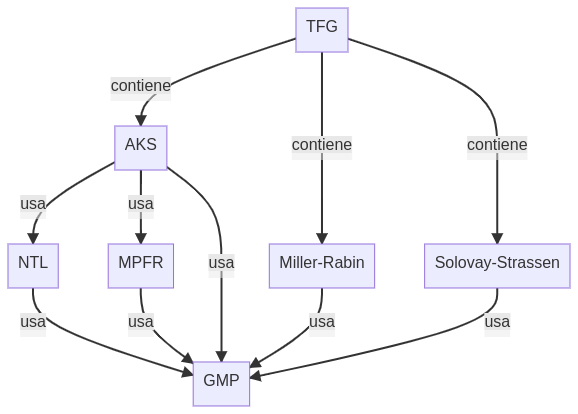
\includegraphics[totalheight=12cm]{img/diagrama-relaciones}
	\caption{Diagrama de relaciones de los componentes del proyecto}
\end{figure}

Todos los tests que se implementan en el proyecto hacen uso de la librería \textbf{GMP} para manejar números de precisión arbitraria. Además el algoritmo \textbf{AKS} hace uso de las librerías \textbf{NTL} (multiplicación de polinomios) y \textbf{MPFR} (cálculo preciso de cotas). Estas dos últimas además hacen uso de \textbf{GMP}. Finalmente tenemos el paquete \textbf{TFG} que incluye todos los tests de primalidad implementados. Ahora vamos a explicar cómo se ha estructurado físicamente el proyecto.\\

El código fuente está incluido todo en una carpeta a la que hemos llamado \textbf{TFG}. Dentro de esta carpeta tenemos varios archivos:

\begin{itemize}
	\item \textbf{.clang-tidy}: Control sobre los warnings que emite Clang-tidy.
	
	\item \textbf{suppressions.txt}: Control sobre los warnings que emite Cppcheck.
	
	\item \textbf{CMakeLists.txt}: Fichero con todas las órdenes necesarias para compilar el proyecto usando CMake.

	\item \textbf{conanfile.py}: Archivo Python donde se añaden las dependencias de Conan.
	
	\item \textbf{graphs.gp}: Archivo de \textbf{gnuplot} que usaremos para generar las gráficas comparativas de los tiempos de ejecución de los tests de primalidad.
\end{itemize}

Luego tenemos varias carpetas:

\begin{itemize}
	\item \textbf{include}: Cabeceras públicas de las funciones (API).
	
	\item \textbf{src}: Implementación de las funciones y cabeceras privadas.
	
	\item \textbf{tests}: Archivos con los tests unitarios.
	
	\item \textbf{examples}: Ejemplos para ejecutar los algoritmos implementados.
	
	\item \textbf{cmake}: Archivos auxiliares que usa el build system.
\end{itemize}

Todas las funciones de la librería se encuentran en un único namespace, llamado \textbf{tfg}, y en el archivo \textbf{include/TFG.hpp}.\\

Las funciones relativas al test \textbf{AKS} se encuentran en el namespace \textbf{tfg::aks}, y los pasos en el namespace \textbf{tfg::aks::steps}. La API se encuentra en el archivo \textbf{include/AKS.hpp}, y la implementación en \textbf{src/AKS.hpp}.\\

Las funciones que actúan como wrapper de las funciones de \textbf{GMP} están en el archivo \textbf{src/GMPWrappers.hpp} (no se exponen como parte de la librería) y las implementaciones en \textbf{src/GMPWrappers.cpp}. Todas estas funciones se encuentran en el namespace \textbf{tfg::gmp}.

\subsection{Comprobar potencia perfecta}

En este apartado vamos a presentar varias decisiones que se han tomado para implementar este algoritmo.\\

A pesar de que probamos que este algoritmo tiene complejidad $O^\sim(\log^4(n))$ y se presentará una posible implementación, la implementación final hará uso de la función ya implementada por la librería \textbf{GMP}.\\

Dicho esto, pasaremos a comprobar las distintas implementaciones.

\subsubsection{Implementación $O(\log^4(n))$}

En esta sección vamos a exponer de manera resumida el código en C++ necesario para implementar esta versión. Tampoco vamos a explicarlo mucho en profundidad, ya que en las siguientes secciones expondremos alternativas más eficientes y rápidas.\\

Primero presentamos la función \textit{isPowerOf}. Esta función toma dos valores $(n, p)$ y comprueba si existe algún $a$ tal que $n = a^p$.\\

\begin{lstlisting}
auto isPowerOf(mpz_class n, size_t p) -> bool {
	auto lower = 0_mpz;
	auto upper = n;
	
	while (lower <= upper) {
		auto middle = mpz_class{(lower + upper) / 2};
		auto value = pow(middle, p);
	
		if (value < n)
			lower = middle + 1;
		else if (value > n)
			upper = middle - 1;
		else
			return true;
	}
	
	return false;
}
\end{lstlisting}

La función puede ser optimizada un poco mejor si la primera cota de la cota superior (upper) es un poco más baja. Por ejemplo $2^{\lfloor \log(n)/p \rfloor + 1}$ sería válida, pero de momento la dejamos más simple.\\

El algoritmo es muy simple. Simplemente calculamos la mitad de ambas cotas, y ese número lo elevamos a $p$. Si el resultado es menor que $n$, actualizamos la cota inferior (lower); si es mayor, actualizamos la superior; y si es igual, devolvemos true. Si el bucle acaba, la búsqueda binaria no ha encontrado el valor, luego devolvemos false.\\

Ahora presentamos el algoritmo \textit{isPerfectPower}. Esta función toma un valor $n$ y comprueba si existen dos valores $a, p > 1$ tales que $n = a^p$.\\

\begin{lstlisting}
auto isPerfectPower(mpz_class n) -> bool {
	auto top = floorLog2(n);

	for (auto p = size_t{2}; p <= top; ++p)
		if (isPowerOf(n, p))
			return true;

	return false;
}
\end{lstlisting}

La función \textbf{floorLog2} se implementa como el número de bits que ocupa $n$ menos 1 (\textit{mpz\_sizeinbase(n.get\_mpz\_t(), 2) - 1}). Sabemos que ese es el top, y luego es simplemente comprobar para cada valor de $p$ si $n = a^p$ para algún $a > 1$.\\

Esta implementación es relativamente simple. Ahora pasaremos a explicar optimizaciones que podemos hacer a esta implementación para reducir la complejidad a $O^\sim(\log^3(n))$, tal y como se explica en \cite{bach_sorenson_1989}, Theorem 3.1.

\subsubsection{Implementación $O^\sim(\log^3(n))$}

En esta implementación simplemente realizaremos algunas pequeñas modificaciones a la anterior para poder reducir la complejidad.\\

En primer lugar, la primera optimización que haremos será reducir la primera cota superior en la función \textit{isPowerOf}. Por tanto, el único cambio es el siguiente:\\

\begin{lstlisting}
auto upper = pow(2_mpz, floorLog2(n) / p + 1);
\end{lstlisting}

De este modo, la complejidad de \textit{isPowerOf} pasa a ser $O(\log^3(n)/p)$, en contraste con la implementación del apartado anterior que era $O(\log^3(n))$. Ahora tenemos que optimizar la función \textit{isPerfectPower}.\\

Para ello, en vez de calcular una cota superior, simplemente vamos a usar el algoritmo de la Criba de Eratóstenes para calcular todos los primos menores que $\log(n)$. Suponiendo que tenemos dicho algoritmo implementado, la nueva versión quedaría tal que así:\\

\begin{lstlisting}
auto isPerfectPower(mpz_class n) -> bool {
	auto primes = eratosthenesSieve(floorLog2(n));
	
	for (auto prime : primes)
		if (isPowerOf(n, p))
			return true;
	
	return false;
}
\end{lstlisting}

La función \textit{eratostheneSieve} básicamente calcula todos los $p \in \N$ primos tales que $p \leq \lfloor \log(n) \rfloor$.\\

Luego simplemente iteramos cada primo y hacemos la comprobación con la búsqueda binaria.\\

Este algoritmo tiene complejidad $O^\sim(\log^3(n))$ \cite{bach_sorenson_1989}.

\subsubsection{Implementación GMP}

La versión que finalmente se ha implementado es la que ya proporciona la librería \textbf{GMP}. Dicha función se llama \textit{mpz\_perfect\_power\_p}. Recibe un único argumento $n$ de tipo \textit{mpz\_t} y devuelve un entero distinto de $0$ si $n$ es una potencia perfecta.\\

La función se ha encapsulado en su correspondiente wrapper llamado \textbf{isPerfectPower} en el namespace \textbf{tfg::gmp}. La implementación es la siguiente:\\

\begin{lstlisting}
auto isPerfectPower(mpz_class const& n) -> bool {
	return mpz_perfect_power_p(n.get_mpz_t()) != 0;
}
\end{lstlisting}

Este algoritmo utiliza el método de Newton para calcular raíces. Una explicación un poco más detallada se puede encontrar en el Apéndice <apéndice implementación potencia perfecta de GMP>.

\subsection{Encontrar menor $r$ tal que $ord_r(n) > \log^2(n)$}

En este paso vamos a calcular el valor de $r$ que luego usaremos en el paso 5. Explicaremos tanto la manera en que calculamos la cota como el cálculo de $ord_r(n)$ de manera eficiente.

\subsubsection{Calcular $\log^2(n)$}

Para calcular esta cota de manera fiable y lo más baja posible, usaremos la librería \textbf{MPFR}, ya que con \textbf{GMP} no podemos asegurar una cota tan precisa. Para calcular la cota, este es el código:\\

\begin{lstlisting}
auto log2Sqr(mpz_class n) -> size_t {
	mpfr_t thresholdMPFR;
	mpfr_init_set_z(thresholdMPFR, n.get_mpz_t(), MPFR_RNDU);
	mpfr_log2(thresholdMPFR, thresholdMPFR, MPFR_RNDU);
	mpfr_sqr(thresholdMPFR, thresholdMPFR, MPFR_RNDU);
	
	return mpfr_get_ui(thresholdMPFR, MPFR_RNDD);
}
\end{lstlisting}

Primero cabe destacar que la cota no debería sobrepasar los 64 bits de capacidad (pues luego tendremos que reservar memoria acorde a esta cota), luego podemos devolver un entero sin signo cuyo valor máximo nunca será menor que la cantidad de memoria del ordenador.\\

Primero inicializamos una variable de tipo \textit{mpfr\_t} (número en coma flotante con precisión arbitraria) con la función \textit{mpfr\_init\_set\_z}, que toma nuestro entero de \textbf{GMP} y lo redondea hacia $+\infty$.\\

Después realizamos \textit{mpfr\_log2} y \textit{mpfr\_sqr} sucesivamente, que son las funciones logaritmo en base $2$ y elevar al cuadrado respectivamente (todo esto reutilizando la misma memoria). Seguimos redondeando a $+\infty$.\\

Finalmente devolvemos la cota que hemos calculado en coma flotante como si fuera un entero redondeado hacia $-\infty$ (o lo que es lo mismo, $\lfloor \log_2(n)^2 \rfloor$).

\subsubsection{Comprobar que $ord_r(n) > \log^2(n)$}

Para este paso, como ya explicamos anteriormente, no necesitamos calcular explícitamente $ord_r(n)$, sino simplemente comprobar que $n^k \neq 1 \mod(r)$ para todo $k \leq \log^2(n)$. Este es el código:\\

\begin{lstlisting}
auto isOrderBiggerThan(mpz_class n, size_t r, size_t threshold) -> bool {
	auto temp = 1_mpz;
	
	for (auto i = std::size_t{1}; i <= threshold; ++i) {
		temp *= n;
		temp %= r;
		
		if (temp == 1)
			return false;
	}
	
	return true;
}
\end{lstlisting}

Las entradas son $n$ (número cuya primalidad queremos testear), $r$ (el valor actual que estamos comprobando) y threshold (cota previamente calculada).\\

Es importante remarcar que, aunque sabemos que la cota es $\log^2(n)$ y, por lo tanto, podríamos calcularla dentro del bucle, es preferible calcularla fuera una vez y pasarla simplemente a esta función cada vez.\\

El algoritmo simplemente comprueba si en algún momento $n^k \equiv 1 \mod(r)$ y, en dicho caso, devolver false (pues el orden entonces es menor que la cota que hemos pasado).\\

Si acabamos el bucle, significa que $ord_r(n) > \log^2(n)$, luego devolvemos true.

\subsubsection{Bucle para probar valores de $r$}

Con las dos funciones anteriores, estamos preparados para ejecutar el segundo paso. Este es el código:\\

\begin{lstlisting}
auto step2(mpz_class n) -> size_t {
	auto const threshold = log2Sqr(n);
	
	for (auto r = threshold + 2;; ++r)
		if (isOrderBiggerThan(n, r, threshold))
			return r;
}
\end{lstlisting}

Lo importante a destacar aquí es que el primer $r$ que probamos es $\log^2(n) + 2$, pues este es el primer $r$ para el que es posible que se cumpla que $ord_r(n) > \log^2(n)$.\\

La razón e que, dado que $n^{\phi(r)} \equiv 1 \mod(r)$ para todo $n, r \geq 1$, si $r \leq \log^2(n) + 1 \Rightarrow ord_r(n) \leq \phi(r) \leq r - 1 \leq \log^2(n)$, luego sería imposible que $ord_r(n) > \log^2(n)$.\\

Más allá de esa aclaración, el código es fácil de entender. Simplemente vamos probando varios valores de $r$ hasta que encontremos uno que cumple la condición, el cual ya sabemos que existe por \autoref{cota_superior_r_log5}.

\subsection{Comprobar si $1 < (a, n) < n$ para algún $a \leq r$}

Este paso consiste simplemente en calcular el máximo común divisor repetidamente para valores de $a \leq r$. El código para ello es el siguiente:\\

\begin{lstlisting}
auto checkGCD(mpz_class n, size_t r) -> bool {
	for (auto a = size_t{2}; a <= r; ++a) {
		auto const result = gmp::gcd(a, n);
	
		if (1 < result && result < n)
			return true;
	}
	return false;
}
\end{lstlisting}

Como dijimos anteriormente, usamos \textbf{size\_t}/\textbf{std::size\_t} para el tipo de $r$ (pues luego lo usaremos para reservar memoria).\\

La función \textit{gmp::gcd} simplemente es un wrapper de la función de \textbf{GMP}, el cual ya explicamos al principio de este capítulo.\\

Si encontramos un $a$ de manera que $1 < (a, n) < n$, devolvemos true. En caso contrario, devolvemos false.

\subsection{Comprobar si $n \leq r$}

Este paso es el más fácil de todos, y ocupará poco espacio en nuestro análisis.\\

En este paso simplemente vamos a añadir la siguiente condición, la cual se encuentra entre el paso $3$ y el paso $5$:\\

\begin{lstlisting}
if (n <= r)
	return true;
\end{lstlisting}

Podemos optimizar esto un poco más si tenemos en cuenta que este paso solo es necesario, ya que la condición $n \leq r$ solo se cumple si $n \leq 5.690.034$, pues $\lceil \log^5(r) \rceil < r$ para todo $n > 5.690.034$.\\

Esta optimización puede ser útil cuando el número de cifras crezca mucho, aunque tampoco va a afectar demasiado, pues volvemos a insistir que la complejidad real está en el paso 5.

\subsection{Comprobar identidades polinómicas}

Este apartado será en el que invirtamos más tiempo, pues es en el que realmente tenemos que optimizar donde sea posible para poder tener un tiempo de ejecución razonable.\\

Lo 4 pasos anteriores no suponen ningún problema de eficiencia con números relativamente grandes. El tener que manejar memoria en este paso puede suponer un auténtico problema si no lo hacemos adecuadamente, pues muchas reservas de memoria pueden resultar en un tiempo de ejecución muy lejos de lo que aspiramos conseguir.\\

En este apartado discutiremos 2 implementaciones posibles. Cada una tiene sus ventajas e inconvenientes, los cuales detallaremos a continuación:\\

\begin{itemize}
	\item \textbf{Implementación directa}. Esta implementación es la más directa, sencilla de integrar en el código fuente (ya que no hace uso de librerías externas) y la que nos da más flexibilidad al tomar distintas decisiones.\\
	
	La mayor desventaja es que será muy complicado lograr una eficiencia parecida a la que otras librerías ya han conseguido, pues mientras que esta implementación se puede realizar en un par de días o tres de desarrollo, optimizarla puede suponer un tiempo innecesariamente largo.\\
	
	Además de lo mencionado, para que el algoritmo sea realmente rápido, habría que implementar la versión de la multiplicación polinómica que hace uso de la \textit{Transformada Rápida de Fourier} (FFT). En nuestro caso usaremos el método clásico para no perder excesivo tiempo en dicha implementación y centrarnos más en las que nos proporciona la librería siguiente.
	
	\item \textbf{NTL}. Esta librería ya tiene implementadas funciones para poder trabajar con anillos de polinomios y módulos, además de haber sido optimizada. Además, la interfaz es en C++, lo cual facilita su integración.\\
	
	Sin embargo esta librería no viene incluida con el manejador de paquetes de Conan, por lo que será necesario instalar dicha librería en el sistema o compilarla a mano, lo cual puede resultar engorroso para el usuario final.
\end{itemize}

Dicho esto, empecemos con el análisis de la implementación del paso 5.

\subsubsection{Cálculo de cota superior para el bucle}

La primera parte del paso es calcular el valor para saber cuántas iteraciones tenemos que realizar. Esta cota es $\lfloor \sqrt{\phi(r)}\log(n) \rfloor$. Para ello, recurriremos de nuevo a la librería \textbf{MPFR} para conseguir una cota lo más fiel y baja posible.\\

Primero necesitamos una implementación para la función $\phi$ de Euler, la cual podemos ver en el siguiente código. Aquí no usamos el tipo de \textbf{GMP}, pues sabemos que $r$ cabe en el tipo \textit{size\_t}:\\

\begin{lstlisting}
auto phi(size_t n) -> size_t {
	auto const top = size_t{std::sqrt(n)};
	auto result = n;

	for (auto p = size_t{2}; p <= top; ++p) {
		if (n % p == 0) {
			while (n % p == 0)
				n /= p;
	
			result -= result / p;
		}
	}
	
	if (n > 1)
		result -= result / n;
	
	return result;
}
\end{lstlisting}

Esta función es una implementación sencilla que simplemente va calculando el valor de $\phi(n)$ a medida que va factorizando $n$. Esta implementación además evita el uso de números en coma flotante, lo cual ayuda a obtener resultados exactos sin recurrir a aproximaciones.\\

Ahora pasamos a explicar la función que calcula la cota. El código para ello es el siguiente:\\

\begin{lstlisting}
auto upperBoundStep5(mpz_class n, size_t r) -> size_t {
	mpfr_t result;
	mpfr_init_set_z(result, n.get_mpz_t(), MPFR_RNDU);
	mpfr_log2(result, result, MPFR_RNDU);
	
	mpfr_t sqrtPhiR;
	mpfr_init_set_ui(sqrtPhiR, phi(r), MPFR_RNDU);
	mpfr_sqrt(sqrtPhiR, sqrtPhiR, MPFR_RNDU);
	
	mpfr_mul(result, result, sqrtPhiR, MPFR_RNDU);
	
	return mpfr_get_ui(result, MPFR_RNDD);
}
\end{lstlisting}

Empezamos calculando $\log(n)$, lo cual lo hacemos fácilmente con las tres primeras líneas. Para ello inicializamos una variable de tipo \textit{mpfr\_t} con $n$ (\textbf{MPFR} admite conversiones desde tipos de \textbf{GMP}) y luego usamos \textit{mpfr\_log2} para aplicarle el logaritmo en base $2$ y así obtener $\log(n)$.\\

Lo siguiente es calcular $\sqrt{\phi(r)}$ en las tres siguientes líneas. Inicializamos otra variable de tipo \textit{mpfr\_t} con el valor de llamar a la función \textit{phi} con $r$, teniendo así $\phi(r)$. Ahora usamos la función \textit{mpfr\_sqrt} para calcularle la raíz cuadrada, obteniendo así $\sqrt{\phi(r)}$.\\

Después calculamos $\sqrt{\phi(r)}\log(n)$ usando la función \textit{mpfr\_mul} y acumulando el resultado en la primera variable que creamos (para no reservar más memoria).\\

Finalmente devolvemos $\lfloor \sqrt{\phi(r)}\log(n) \rfloor$ usando el resultado de la llamada a \textit{mpfr\_get\_ui}, que devuelve el valor del resultado como un entero sin signo y redondeando hacia $-\infty$.\\

Ahora vamos a pasar a explicar las implementaciones del bucle principal del algoritmo. Es solo esta parte en la que divergen varias implementaciones en todo el algoritmo. Esta separación nos servirá luego para poder comparar ambas implementaciones y ver las ventajas de una sobre la otra.\\

Destacar que ambas implementaciones residen en el namespace \textbf{tfg::aks::steps::impl} y están expuestas públicamente. La primera se llama \textit{step5Direct}, y la segunda \textit{step5NTL}. En la implementación final se usa por defecto la segunda por ser más eficiente.

\subsubsection{Bucle: Implementación Directa}

Ahora vamos a centrarnos en cómo podríamos hacer una implementación directa sin hacer uso de librerías externas para el bucle principal del algoritmo \textbf{AKS}.\\

Para ello necesitamos implementar la operación principal de la identidad: exponenciación rápida de un polinomio módulo otro polinomio y un entero. Esta operación puede parecer aparentemente sencilla, pero requiere de un buen manejo de la memoria para no estar reservando memoria constantemente en cada iteración del bucle.\\

Vamos a presentar entonces dos clases que nos ayudarán a la hora de la implementación:

\begin{itemize}
	\item \textbf{AKSCoefficient}: Esta clase es simplemente un wrapper de \textit{mpz\_class} para trabajar con aritmética modular más fácilmente.\\
	
	El único atributo de dichos objetos es una variable de tipo \textit{mpz\_class}, donde las operaciones de suma, resta y multiplicación se han adaptado al anillo $\Z_n$.\\
	
	Además, para que todos los objetos de dicha clase tengan el mismo módulo, se ha añadido una variable estática de clase (común a todos los objetos) que indicará el anillo en el que nos encontramos.
	
	\item \textbf{AKSPolynomial}: Esta clase representa un polinomio con coeficientes en $\Z_n$ y módulo $X^r - 1$ o, dicho de otro modo, el anillo $\Z_n[X]/(X^r - 1)$. Agruparlo así nos servirá para controlar mejor el uso de memoria.\\
	
	Consta de tres atributos:
	
	\begin{itemize}
		\item Dos buffers de tamaño $2r$. Uno para almacenar los coeficientes del polinomio. El otro es un buffer auxiliar que nos servirá para evitar reservas de memoria repetidas cada vez que hagamos una operación sobre los polinomios.
		
		\item Un entero sin signo indicando el grado actual del polinomio.
	\end{itemize}
	
	Además, hay una variable estática de clase que indicará el grado del polinomio que marca el módulo (si el polinomio es $X^r - 1$, nosotros guardamos el valor de $r$).
\end{itemize}

Para ambas clases implementaremos lo justo para poder usarlas con el algoritmo \textbf{AKS}, y además no estarán expuestas en la interfaz pública, por lo que no necesitamos una API extremadamente versátil.\\

La implementación de \textbf{AKSCoefficient} es simplemente un wrapper con las operaciones elementales adaptadas al anillo $\Z_n$, por lo que no vamos a ocupar mucho tiempo en ella.\\

Decir que los operadores que se implementan son +=, -= y *=. Esto es para evitar que se hagan muchas reservas de memoria y simplemente actualizar los valores. Además se implementa el operador == para poder comparar dos objetos de esta clase, constructores que aceptan variables de tipo \textit{mpz\_class} y una pareja getter/setter para cambiar el módulo del anillo, es decir, indicar en qué $\Z_n$ estamos.\\

La clase \textbf{AKSPolynomial} es la que va a hacer el trabajo pesado, pues es la que se va a encargar de implementar las operaciones polinómicas. Vamos a indicar varias características de esta clase:

\begin{itemize}
	\item Una característica importante de esta clase es que no se puede copiar. Tiene el constructor y la asignación por copia eliminados explícitamente. Esto nos va a ayudar a que no se hagan copias accidentalmente.
	
	\item Tiene un constructor que acepta dos variables de tipo \textbf{AKSCoefficient}, que indican los dos primeros coeficientes. Esto es porque en el algoritmo solo necesitamos construir polinomios de esa manera y no con tantos coeficientes como queramos.
	
	\item Los únicos operadores que se implementan son -= y *=. El primero acepta una variable de tipo \textbf{AKSCoefficient} (básicamente restar un escalar al polinomio). El segundo acepta otro polinomio, y es donde se implementará la operación de multiplicación de polinomios.
	
	\item Se implementa la operación \textit{pow}, que acepta una variable de tipo \textit{mpz\_class} y eleva el polinomio a dicho valor. Además acepta un segundo parámetro que es donde se guardará el resultado de la operación (esto con el fin de evitar reservar memoria repetidas veces).
\end{itemize}

Empezamos viendo la operación \textit{pow}. El código es el siguiente:\\

\begin{lstlisting}
auto AKSPolynomial::pow(mpz_class exp, AKSPolynomial& result) const -> void {
	result.setCoefficient(0, 1_mpz);
	result.m_currentDegree = 0;
	
	for (auto const& bit : exp.get_str(2))
	{
		result *= result;
		if (bit == '1')
			result *= *this;
	}
}
\end{lstlisting}

El algoritmo simplemente va tomando los bits del número que se le pasa con la función \textit{get\_str}. Los bits se recorren de más significativo a menos. Simplemente elevamos al cuadrado en cada iteración el resultado y, si el bit es $1$, multiplicamos por el valor que estamos elevando. Este algoritmo es bien conocido y realiza $O(\log(n))$ multiplicaciones.\\

Ahora vamos a presentar una función auxiliar, \textit{adjustDegree}, que sirve para adaptar el grado del polinomio:\\

\begin{lstlisting}
auto AKSPolynomial::adjustDegree() -> void {
	while (getCoefficient(getDegree()) == 0_mpz && getDegree() > 0)
		--m_currentDegree;
}
\end{lstlisting}

Las funciones \textit{getCoefficient} y \textit{getDegree} son getters para obtener un coeficiente específico y obtener el grado del polinomio respectivamente.\\

Simplemente va actualizando el grado del polinomio hasta que se encuentra un coeficiente distinto de $0$ o llega al grado $0$.\\

La siguiente operación que vamos a presentar es la división del polinomio por el módulo:\\

\begin{lstlisting}
auto AKSPolynomial::dividePolMod() -> void {
	if (getDegree() >= getModuleDegree()) {
		for (auto i = getDegree(); i >= getModuleDegree(); --i)
			m_coeffs[i - getModuleDegree()] += getCoefficient(i);
		
		m_currentDegree = getModuleDegree() - 1;
	}
	adjustDegree();
}
\end{lstlisting}

Antes de explicar la función, destacar que la función \textit{getModuleDegree} devuelve el grado del polinomio $X^r - 1$, pues para el algoritmo no necesitamos el polinomio entero y podemos realizar ciertas optimizaciones basadas en ello. La variable \textit{m\_coeffs} es el buffer que contiene los coeficientes.\\

Básicamente, lo que hacemos es aplicar el algoritmo clásico de división de polinomios. Como sabemos que el polinomio siempre es de la forma $X^r - 1$, podemos simplemente actualizar los $n - r$ primeros coeficientes desde el de más grado hasta el de menos. Finalmente reajustamos el grado del polinomio resultante. De este modo, la eficiencia es $O(n - r)$ o $O(r)$ teniendo en cuenta que el polinomio siempre será de grado $O(r)$.\\

Finalmente vamos a presentar la multiplicación. Cabe destacar que aquí usamos el algoritmo elemental. Para conseguir una mejor eficiencia será necesario usar la versión que hace uso de la \textit{Transformada Rápida de Fourier}. Esto no lo haremos aquí ya que puede ser complicado implementarla correctamente y las próximas versiones ya harán ese trabajo por nosotros.\\

\begin{lstlisting}
auto AKSPolynomial::operator*=(AKSPolynomial const& rhs) -> AKSPolynomial& {
	auto const newDegree = getDegree() + rhs.getDegree() + 1;
	
	for (auto i = std::size_t{0}; i <= newDegree; ++i)
		m_coeffsAux[i] = 0_mpz;
	
	for (auto i = std::size_t{0}; i <= getDegree(); ++i) {
		for (auto j = std::size_t{0}; j <= rhs.getDegree(); ++j) {
			auto product = getCoefficient(i);
			product *= rhs.getCoefficient(j);
			m_coeffsAux[i + j] += product;
		}
	}
	
	m_currentDegree = newDegree;
	std::swap(m_coeffs, m_coeffsAux);
	
	dividePolMod();
	
	return *this;
}
\end{lstlisting}

Explicamos cada paso con detalle:

\begin{enumerate}
	\item Primero calculamos el grado final del polinomio resultante (la suma de ambos grados más $1$).
	
	\item Actualizamos los valores del buffer auxiliar, \textit{m\_coeffsAux} a $0$ (preparando el terreno para acumular el resultado).
	
	\item Bucle doble donde básicamente aplicamos el algoritmo elemental de multiplicación de polinomios y acumulamos el resultado en el buffer auxiliar.
	
	\item Actualizamos el grado del polinomio actual al del producto.
	
	\item Intercambiamos los buffers, de modo que el buffer principal contenga el resultado de la multiplicación.
	
	\item Finalmente aplicamos la división por el módulo, la cual ya ajusta el grado del resultado final.
\end{enumerate}

La parte que deberíamos optimizar es el bucle anidado donde realizamos el algoritmo de multiplicación, pero no lo haremos en este apartado ya que será complicado hacerlo correctamente.\\

Finalmente, y haciendo uso de lo que acabamos de explicar, podemos implementar el quinto paso de la siguiente manera:\\

\begin{lstlisting}
auto step5Direct(mpz_class n, size_t r) -> bool {
	auto const top = calculateUpperBound(n, r);
	
	detail::AKSCoefficient::setModule(n);
	detail::AKSPolynomial::setModuleDegree(r);
	
	auto lhs = detail::AKSPolynomial{};
	auto rhs = detail::AKSPolynomial{};
	
	auto temp = detail::AKSPolynomial{0_mpz, 1_mpz};
	
	temp.pow(detail::AKSCoefficient::getModule(), rhs);
	
	for (auto a = std::size_t{1}; a <= top; ++a) {
		temp.setCoefficient(0, mpz_class{a});
		temp.pow(detail::AKSCoefficient::getModule(), lhs);
		lhs -= mpz_class{a};
		
		if (lhs != rhs)
			return true;
	}
	
	return false;
}
\end{lstlisting}

Antes de explicar cada paso en detalle, es importante aclarar que la identidad que vamos a comprobar la vamos a modificar ligeramente. En vez de comprobar $(X + a)^n \equiv X^n + a \mod(X^r - 1, n)$, vamos a comprobar $(X + a)^n - a \equiv X^n \mod(X^r - 1, n)$. Esto nos permite evitar calcular el polinomio de la parte derecha en cada iteración, ya que no dependerá de la variable de iteración $a$. Ahora explicamos en detalle cada paso:

\begin{enumerate}
	\item Primero calculamos la cota del bucle con la función \textbf{calculateUpperBound}.
	
	\item Indicamos a las clases el módulo $(X^r - 1, n)$ en el que vamos a trabajar.
	
	\item Creamos los dos polinomios que usaremos para comprobar las identidades: \textit{lhs} para $(X + a)^n - a$ y \textit{rhs} para $X^n$. Además creamos uno extra que nos servirá para almacenar el resultado de elevar la parte izquierda y no reservar memoria repetidas veces.
	
	\item Almacenamos en \textit{rhs} el resultado de $X^n \mod(X^r - 1, n)$.
	
	\item Empezamos el bucle, y en cada iteración, almacenamos en \textit{lhs} el resultado de $(X + a)^n - a \mod(X^r - 1, n)$. Comparamos \textit{lhs} con \textit{rhs}, y devolvemos true si no coinciden.
	
	\item Si llegamos al final del bucle, devolvemos false (Es decir, que se han cumplido las identidades).
\end{enumerate}

La complejidad de esta implementación está entre $O^\sim(\log^8(n))$ y $O^\sim(\log{31/2}(n))$ (según el valor de $r$). Esto se debe a que la multiplicación de enteros viene dada por la librería \textbf{GMP}, que implementa la dicha operación con complejidad $O^\sim(\log(n))$; y porque el algoritmo de multiplicación de polinomios implementado sin uso de librerías externas es $O^\sim(r^2\log(n))$.

\subsubsection{Bucle: Implementación con NTL}

En este apartado nos vamos a centrar en implementar el paso 5 haciendo uso de la librería \textbf{NTL}.\\

Esta implementación hace uso de algoritmos para realizar la multiplicación de polinomios con complejidad $O^\sim(nm)$ en vez de $O^\sim(n^2m)$, como en el apartado anterior.\\

Presentamos entonces una implementación del paso 5 haciendo uso de la librería \textbf{NTL}:\\

\begin{lstlisting}
auto step5NTL(mpz_class n, size_t r) -> bool {
	auto const top = calculateUpperBound(n, r);
	
	auto const nNTL = NTL::conv<NTL::ZZ>(n.get_str().c_str());
	NTL::ZZ_p::init(nNTL);
	
	auto const module = NTL::ZZ_pXModulus{NTL::ZZ_pX{r, 1} - 1};
	
	auto const rhs = [&nNTL, &module] {
		auto result = NTL::ZZ_pX{1, 1};
		NTL::PowerMod(result, result, nNTL, module);
		
		return result;
	}();
	
	for (auto a = std::size_t{1}; a <= top; ++a) {
		auto lhs = NTL::ZZ_pX{1, 1};
		lhs += a;
		NTL::PowerMod(lhs, lhs, nNTL, module);
		lhs -= a;
		
		if ((lhs != rhs) != 0)
			return true;
	}
	
	return false;
}
\end{lstlisting}

Primero, al igual que en la implementación anterior, calculamos la cota superior del bucle haciendo uso de la función \textit{calculateUpperBound}.\\

Después convertimos la entrada (entero de \textbf{GMP}, \textit{mpz\_class}) a un entero de \textbf{NTL}, \textit{NTL::ZZ}, para poder usarlo en los algoritmos de esta librería. Hecho eso, inicializamos el módulo $\Z_n$ con la llamada a \textit{NTL::ZZ\_p::init}. Esto hará que todas las operaciones en enteros sean módulo $n$.\\

Ahora declaramos el polinomio $X^r - 1$ como el módulo que usaremos para exponenciar.\\

Después calculamos $X^n \mod(X^r-1, n)$ con la función \textit{NTL::PowMod}. El segundo parámetro es el polinomio a exponenciar (base). El tercer parámetro es el exponente. El cuarto parámetro es el polinomio cuyo módulo vamos a aplicar.El resultado se guarda en el primer parámetro.\\

Finalmente ejecutamos el bucle, y en cada iteración calculamos $(X + a)^n - a \mod(X^r-1, n)$. Si alguna identidad no se cumple, devolvemos true.\\

Finalmente, si llegamos al final del bucle, devolvemos false (pues todas las identidades se han cumplido).\\

La complejidad de esta implementación está entre $O^\sim(\log^6(n))$ y $O^\sim(\log{21/2}(n))$ (según el valor de $r$). Esto se debe a que la multiplicación de enteros viene dada por la librería \textbf{GMP}, que implementa la dicha operación con complejidad $O^\sim(\log(n))$; y porque el algoritmo de multiplicación de polinomios implementado por \textbf{NTL} tiene complejidad $O^\sim(r\log(n))$.

\subsection{Paso 6: Devolver true}

Este paso simplemente se implementa como una función a parte para ser más fiel al algoritmo original y estar en concordancia con el resto de pasos. Consiste en una función que devuelve true.

\section{Comparación Implementación Directa/NTL}

En esta sección vamos a justificar con resultados gráficos la elección de usar la librería externa \textbf{NTL} a la hora de elegir una implementación definitiva del paso $5$ del algoritmo \textbf{AKS}.\\

Como ya explicamos anteriormente, este paso es el único en el que usamos implementaciones distintas, por lo que el resto de pasos serán comunes en la comparación y solo mediremos el tiempo de ejecución del quinto paso.\\

Para la comparación vamos a usar los mayores primos que ocupan una cantidad determinada de bits (desde $2$ bits hasta $16$ bits). Nuestro conjunto de prueba será el siguiente:

\[ \{ 3, 7, 13, 31, 61, 127, 251, 509,
1021, 2039, 4093, 8191, 16381, 32749,
65521 \} \]

No usamos primos más grandes porque, como veremos en las gráficas, el tiempo que invierte la implementación directa es muy alto para números pequeños.\\

No usamos números compuestos porque necesitamos comparar la eficiencia del paso $5$, el cual se ejecuta por completo cuando la entrada se trata de un número primo. Es por ello que aquí no tiene mucho sentido usar números compuestos. Por esta razón, en la comparación solo vamos a ejecutar los pasos $2$ y $5$, ya que necesitamos el valor de $r$ calculado en el segundo paso para poder ejecutar el quinto.

Además de presentar los tiempos de ejecución de ambas implementaciones, también vamos a representar las gráficas de las eficiencias teóricas ajustadas con la función \textit{fit} de \textit{gnuplot}.\\

Ambos ejes de las gráficas están en escala logarítmica en base $2$, para que se puedan apreciar mejor los resultados.\\

Esta gráfica muestra los tiempos de ejecución de la implementación directa junto con sus eficiencias teóricas.

\begin{figure}[H]
	\centering
	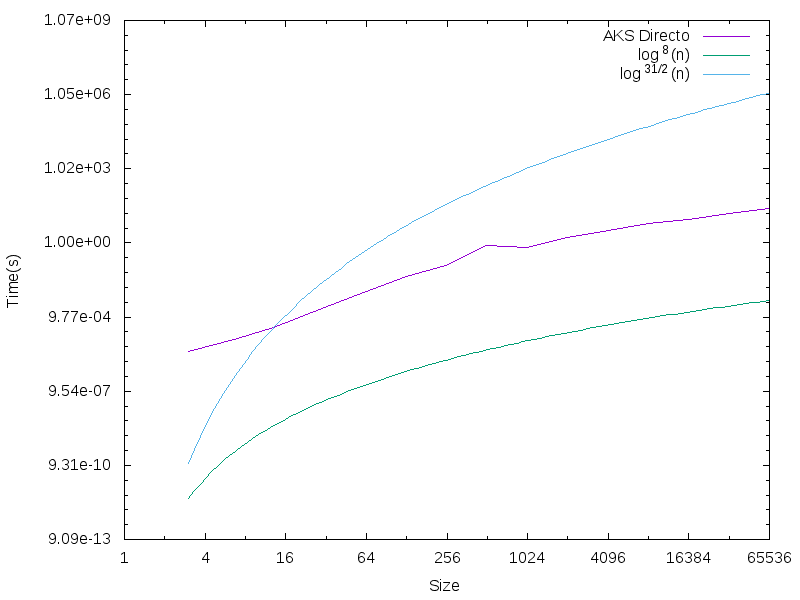
\includegraphics[totalheight=12cm]{img/graphs/aks-direct-mean}
	\caption{Gráfica AKS con implementación directa}
\end{figure}

Esta gráfica muestra los tiempos de ejecución de la implementación usando \textbf{NTL} junto con sus eficiencias teóricas.

\begin{figure}[H]
	\centering
	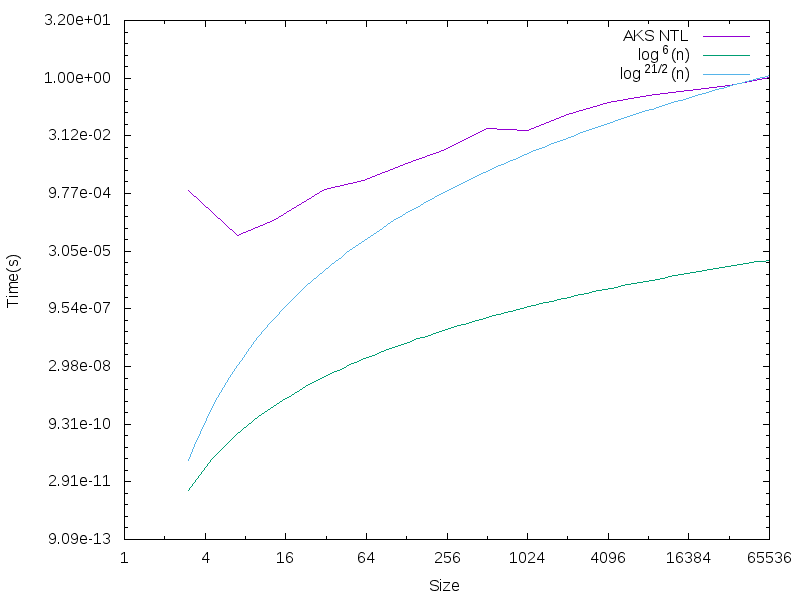
\includegraphics[totalheight=12cm]{img/graphs/aks-ntl-mean}
	\caption{Gráfica AKS usando NTL}
\end{figure}

Finalmente mostramos la comparación de ambas implementaciones.

\begin{figure}[H]
	\centering
	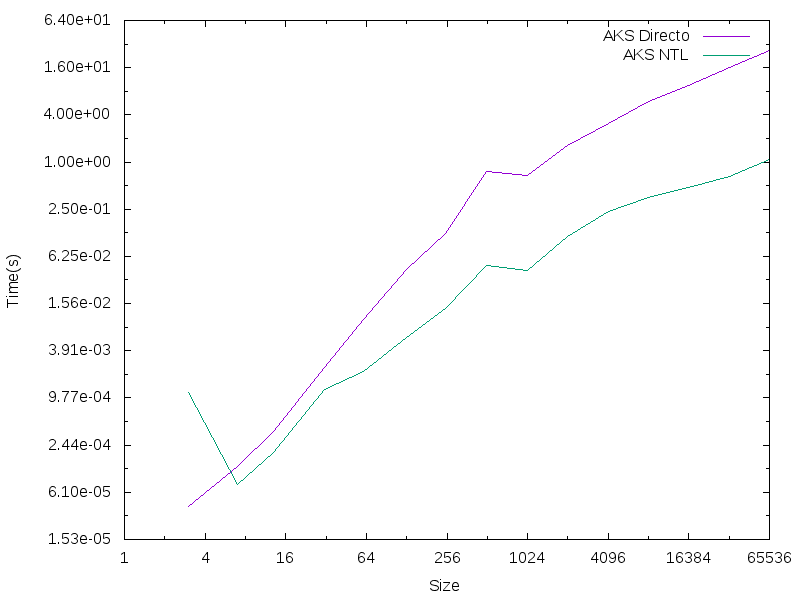
\includegraphics[totalheight=12cm]{img/graphs/aks-mean}
	\caption{Comparación ambas implementaciones AKS}
\end{figure}

Como podemos comprobar, el tiempo de ejecución de la implementación directa es mucho mayor que la implementación usando la librería \textbf{NTL}. Esto es debido al algoritmo de multiplicación polinómica usado en ambos casos, lo cual resalta su importancia a la hora de implementar el algoritmo \textbf{AKS}.\\

Puesto que la implementación usando \textbf{NTL} es superior, será la que usaremos en el siguiente apartado para comparar el algoritmo \textbf{AKS} con los tests probabilísticos de \textit{Miller-Rabin} y \textit{Solovay-Strassen}.

\endinput
%------------------------------------------------------------------------------------
% FIN DEL CAPÍTULO. 
%------------------------------------------------------------------------------------
